\section{Deadlocks und Priority Inversion}

Bei überlappender oder zyklischer Belegung von Betriebsmitteln (Ressourcen) können Verklemmungen (Deadlocks) auftreten.
\textbf{Race Condition}: unerwünschtes Wettrennen mehrere Tasks um gleichzeitigen Zugriff auf Ressource.
Ein Deadlock ist immer die Folge eines logischen Programmfehlers!

Eine Möglichkeit um Deadlocks erkennen zu können ist der Prozessfahrplan:

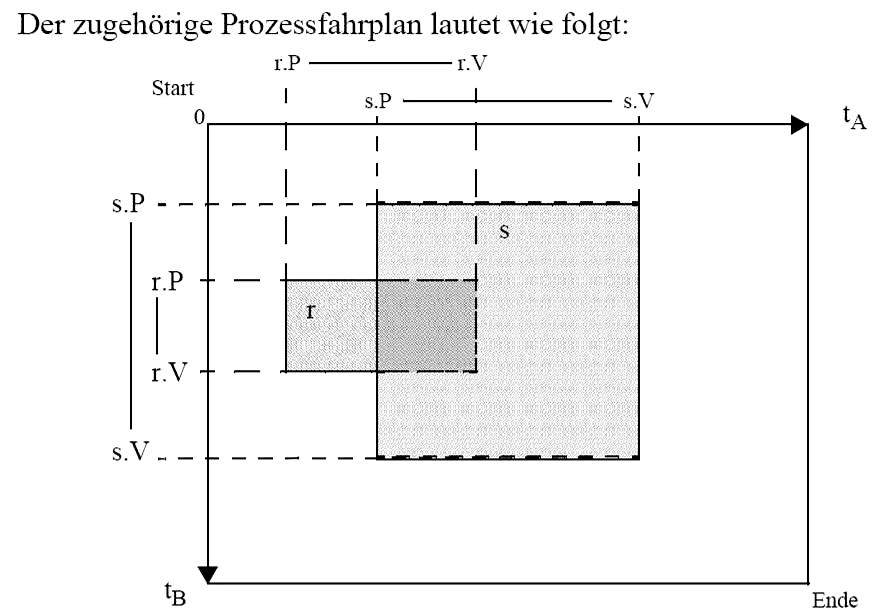
\includegraphics[width=\linewidth]{Prozessfahrplan.png}

Methoden zum verhindern von Deadlocks:

\begin{itemize}
    \itemsep-.5em 
    \item Eliminate the \textit{no preemption} deadlock condition: Task must release already acquired resources if a new request is denied. Task must then initiate a new request, including both the new resource and all previously held resources.
    \item Eliminate the \textit{hold and wait} deadlock condition: Task requests at one time all needed resources; it can begin execution only when every resource from the request set is granted.
    \item Eliminate the \textit{circular wait} deadlock condition: All tasks shall request the resources in the very same numbering according to an imposed ordering on the resources.
\end{itemize}


\subsection{Priority Inversion}

Wenn ein Low priority Task eine Resource blockiert welche von eine high Priority Task benötigt wird.

Bounded Priority Inversion:

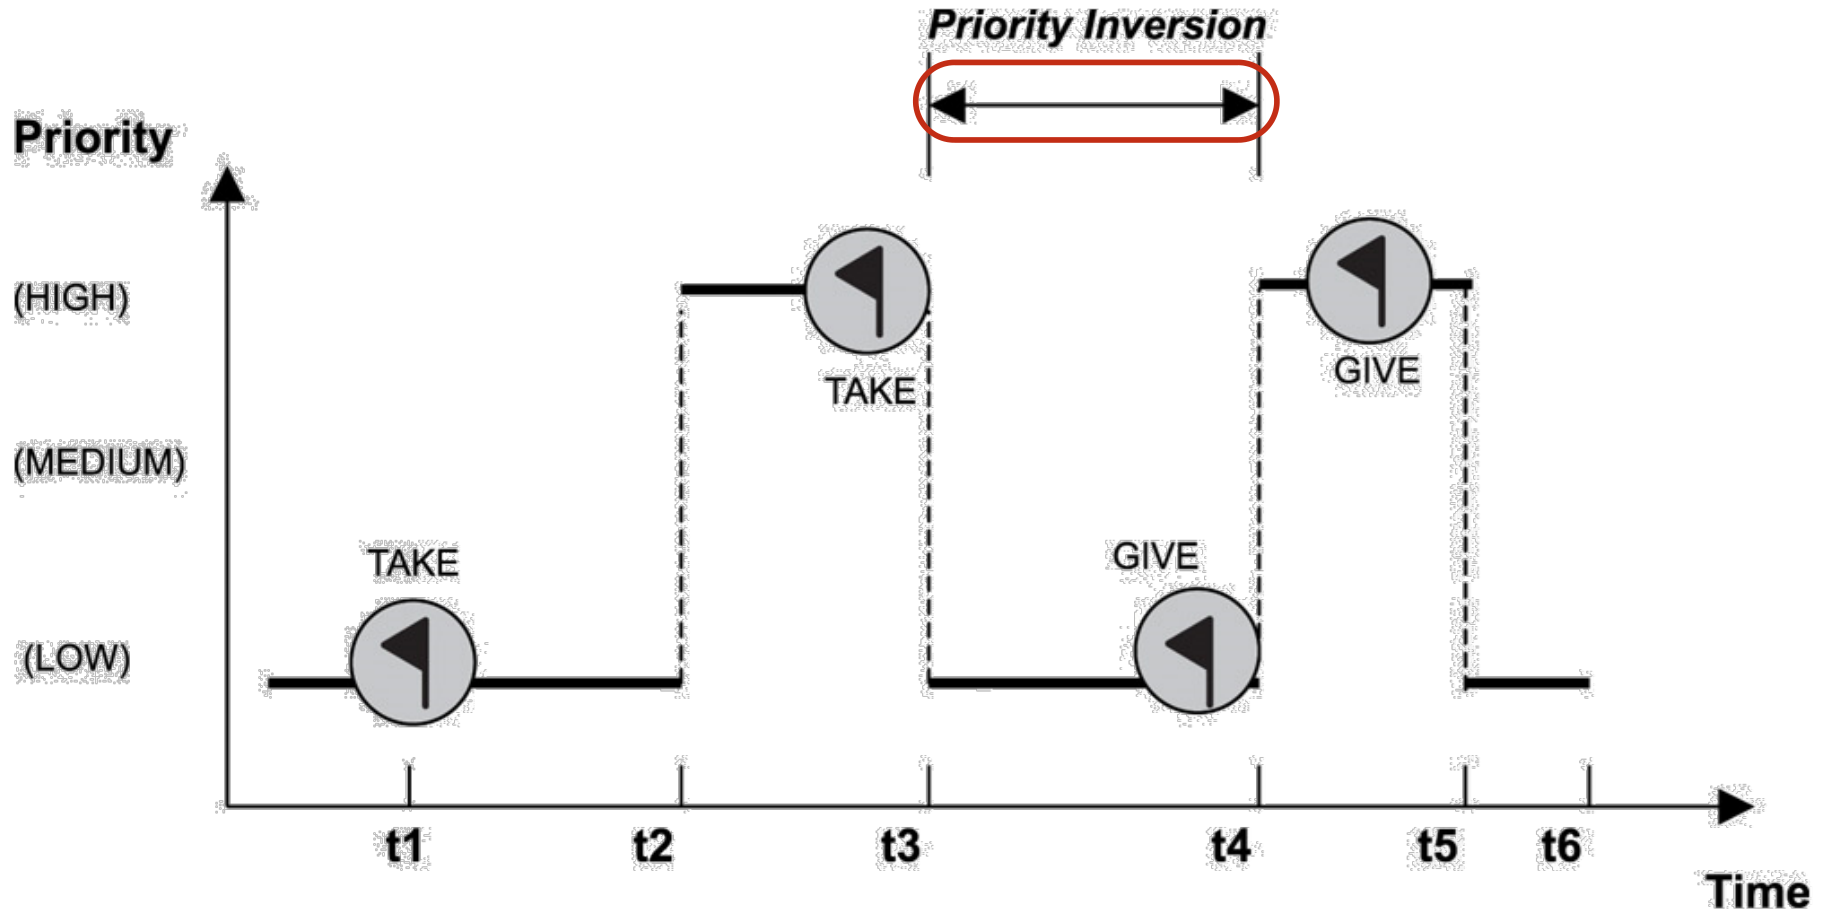
\includegraphics[width=\linewidth]{BoundedPriorityInversion.png}

Unbounded Priority Inversion:

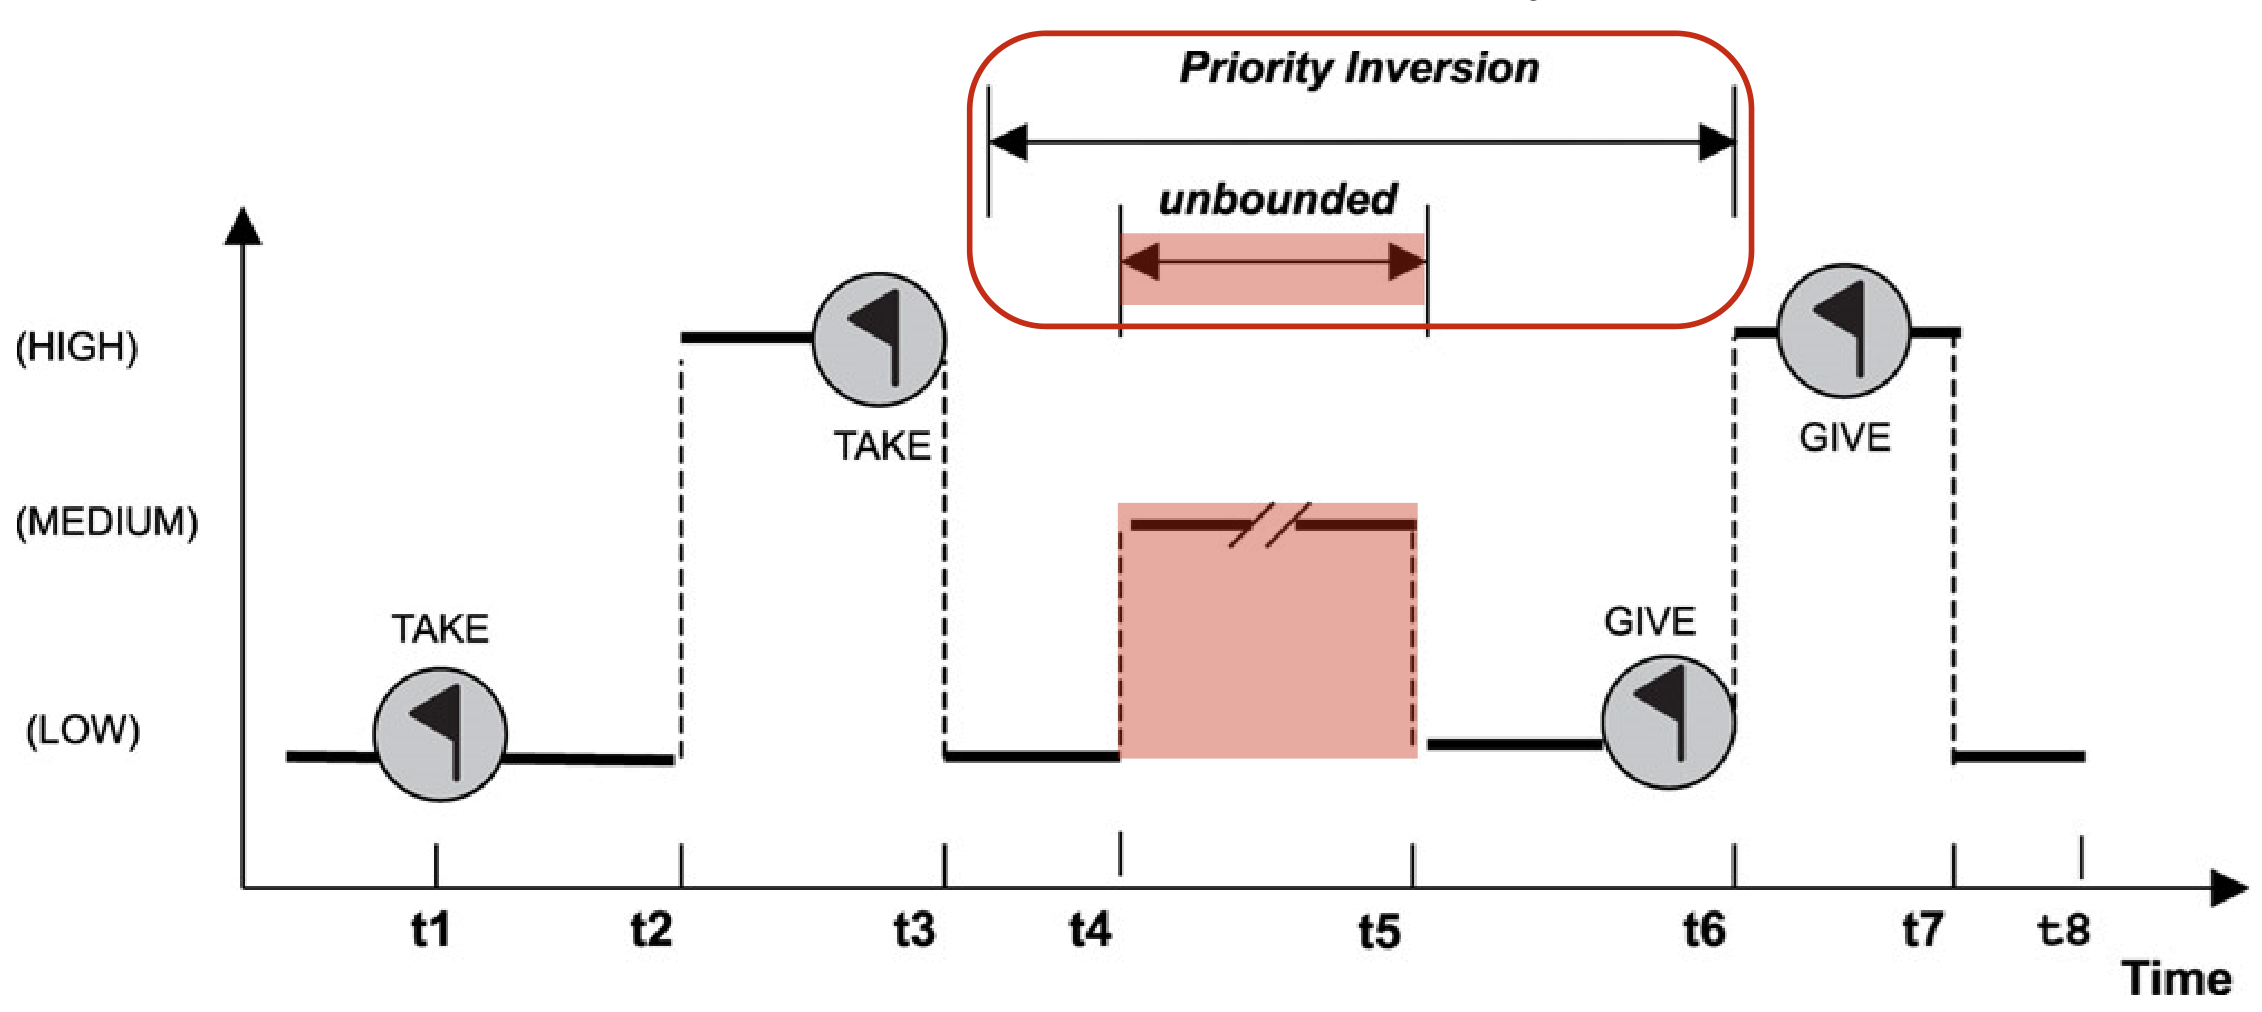
\includegraphics[width=\linewidth]{UnboundedPriorityInversion.png}

\subsubsection{Priority Inheritance Protocol (PIP)}

Erhöht die priorität des LPT zu der des HPT damit die Resource schneller freigegeben wird.

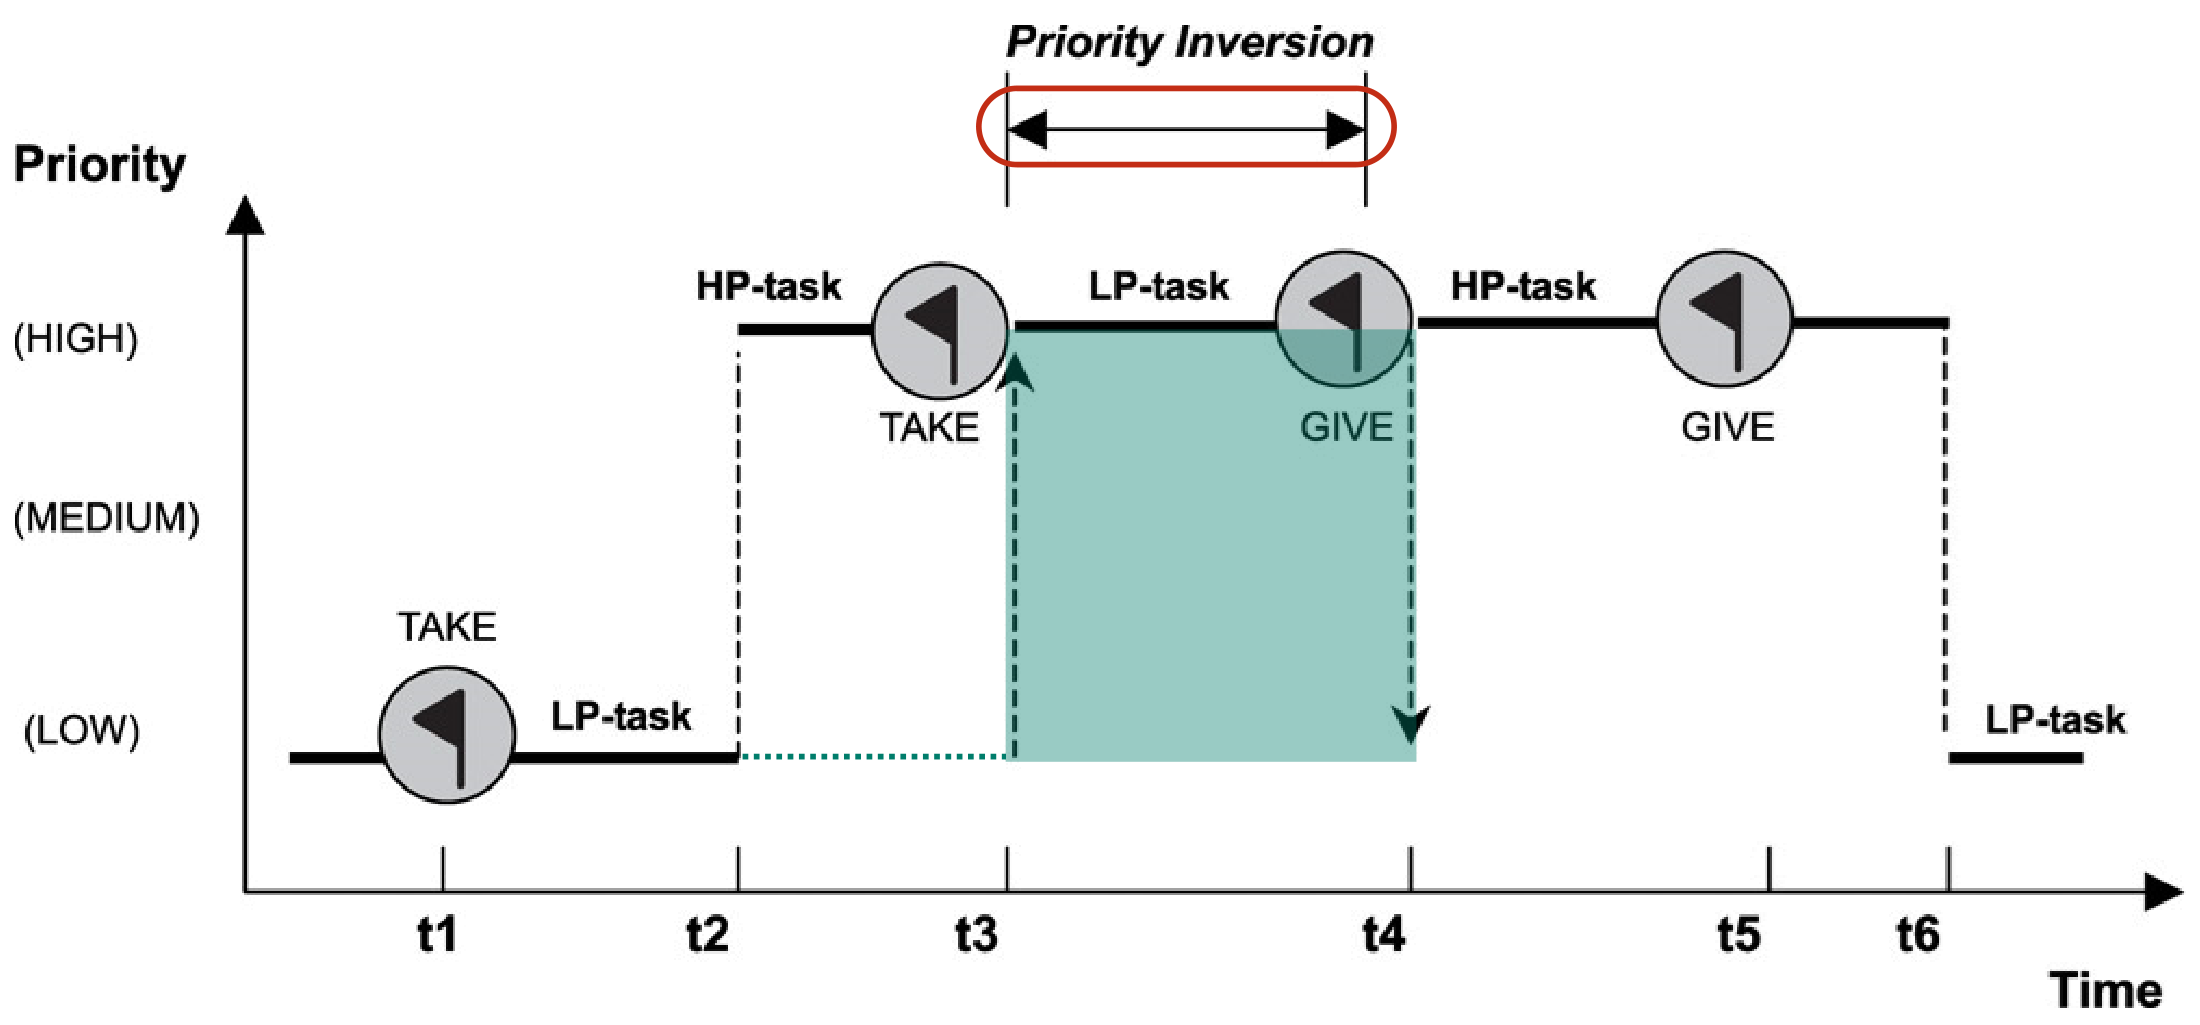
\includegraphics[width=\linewidth]{PriorityInheritanceProtocol.png}

\subsubsection{Transitive Priority Promotion}

Der "transitive" Teil bedeutet, dass diese Prioritätsbeförderung nicht nur zwischen zwei Tasks stattfindet, sondern sich über mehrere Ebenen von wartenden Tasks ausbreiten kann.

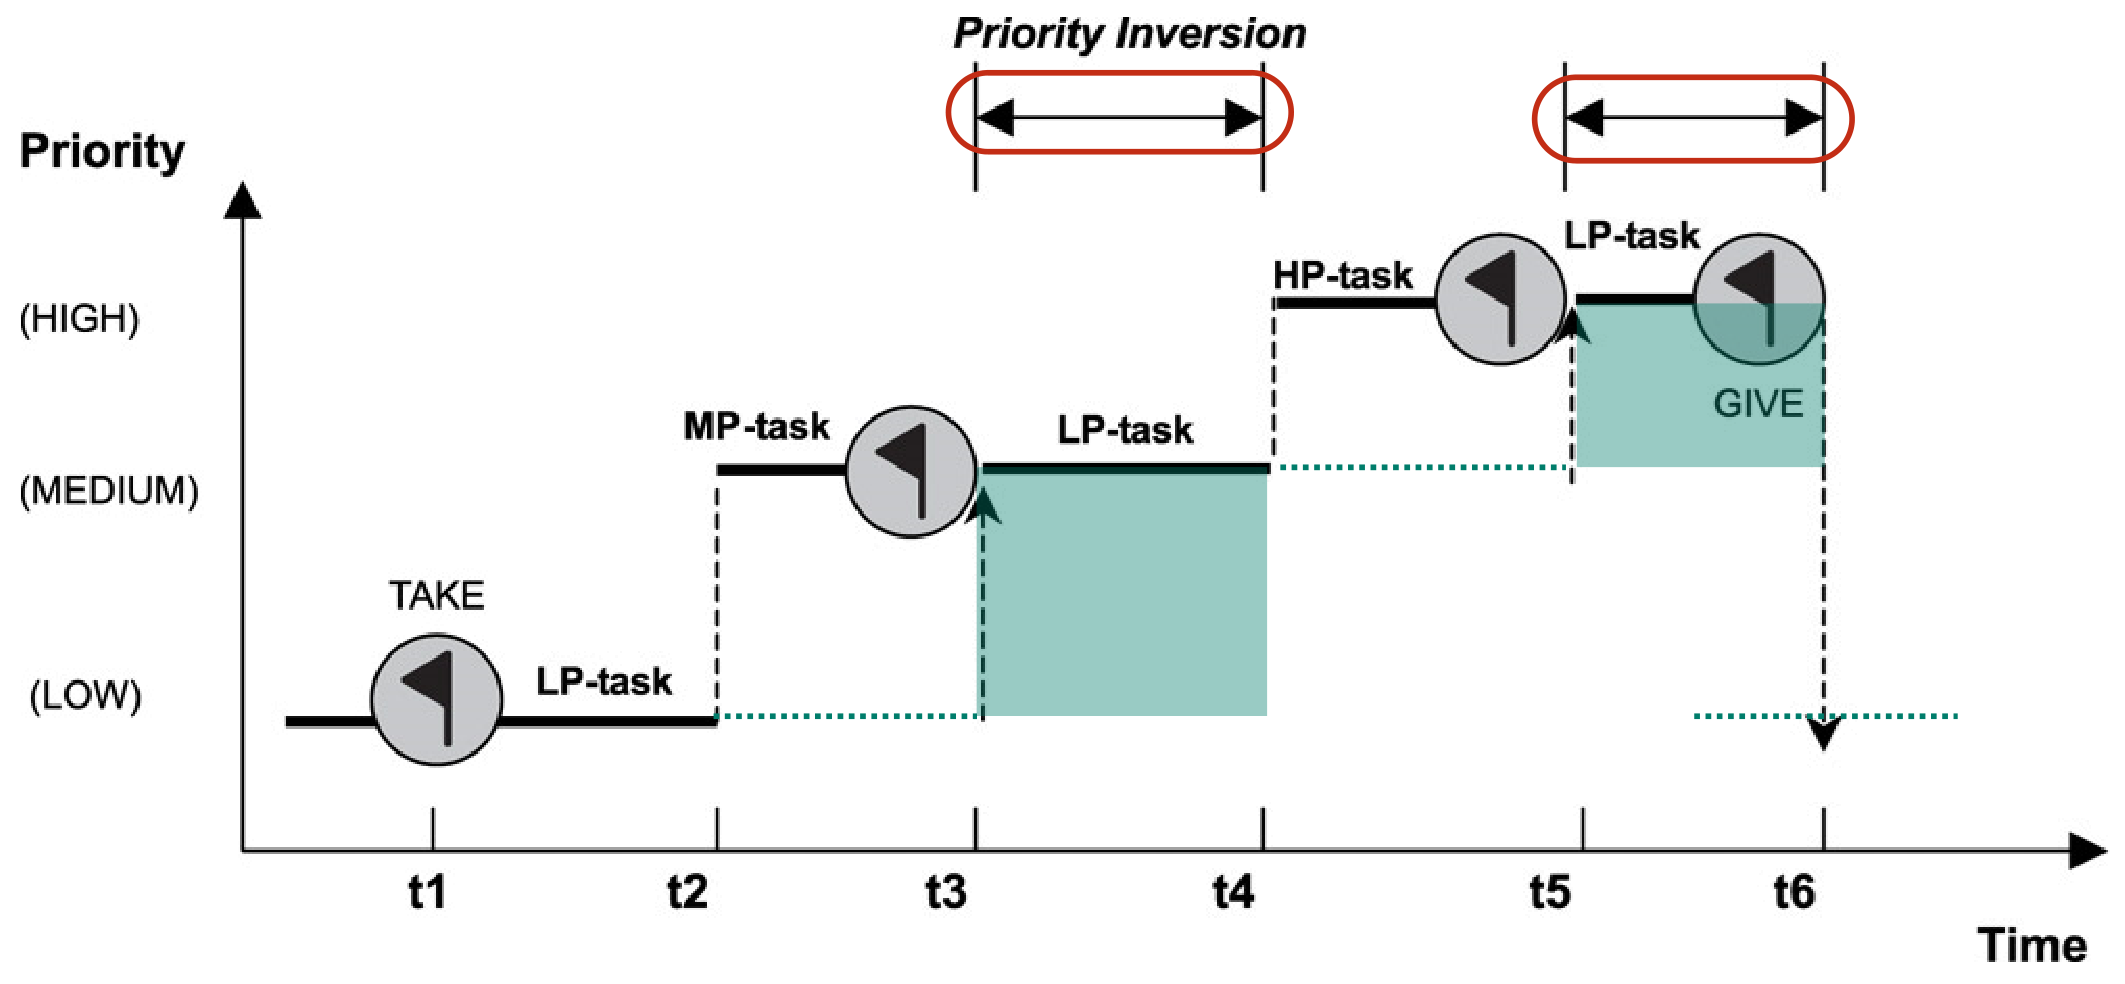
\includegraphics[width=\linewidth]{TransitivePriorityPromoton.png}

\subsubsection{Priority Ceiling Protocol (PCP)}

\underline{Variante 1, Regeln:}

Task erhält direkt die Highest priority ceiling Priorität der Resource.

\begin{itemize}
    \itemsep-.5em 
    \item If resource locked, task blocks.
    \item If resource free, task takes and locks it; task's priority raised to resource's priority ceiling.
    \item When resource released, task's priority is assigned to highest priority of remaining resources held.
\end{itemize}

\underline{Variante 2, Regeln:}

Current priority ceiling = highest priority ceiling of all resources in use at given time.

\begin{itemize}
    \itemsep-.5em 
    \item If resource locked, task blocks
    \item If resource free and task's priority > current priority ceiling, task takes and locks it, else
    \item If current priority ceiling stems from another resource the task currently already holds, task can also take and lock this resource, else task blocks.
    \item Blocked task passes on its priority to other blocking task (priority inherited if higher); if that other blocking task releases a resource, it assumes highest priority among all tasks still blocked by resources held; if not blocking any other task, task returns to normal priority.
\end{itemize}


